\chapter{Event Reconstruction}
\label{ch:RecoCal}

The most basic form of raw data collected is a vector of hits above threshold. The MC simulation described in chapter \ref{ch:Simulation} also outputs events in this format. However, these objects by themselves are not very useful; instead, a certain level of reconstruction is required before real physics can be studied. The first major step in this process is to apply calibration so that the hits can be translated into a set of energy depositions, consistent throughout and across both detectors. Any number of algorithms can then be applied to create new objects or search for features, including tracks, the event vertex, or particle identifiers (PIDs). This chapter describes the calibration and elements of the reconstruction chain relevant to the NC disappearance analysis.

\section{Calibration}

The purpose of calibration is to ensure a uniform detector response throughout each and across both detectors. This is done in two major steps, a relative and absolute calibration. The relative calibration accounts for threshold effects and attenuation across a single cell. It is designed to create a uniform response throughout a cell and across a single detector. The absolute calibration creates a scale factor for each detector to convert the calibrated PE scale from the relative calibration into an energy unit. This section follows the SA notes in reference \cite{ref:TNCalib}.

The relative calibration is designed to convert the PE signal output from the electronics into a calibrated unit, such that two equal signals from any two detector locations mean equal true energy deposited. This part of the calibration accounts for threshold effects and attenuation in the WLS fibers, outputting a corrected PE value, the PECorr.

Hits from through-going cosmic ray muons, or muons that enter and exit the detector without stopping, are used for the relative calibration. The WindowTrack algorithm, a fast algorithm that fits straight lines through hits \cite{ref:RecoWinTrack}, is used to produce 3D tracks from the cosmic ray events, and only those with a successful reconstruction are used. Within these events, only tricell hits are used for the calibration procedure. A tricell hit is defined as a hit in cell $i$ within a given plane that also has hits in cells $i+1$ and $i-1$. Under special circumstances (low statistics, too many dead neighboring cells) different hits are used for a particular cell. The path length of the cosmic traveling through the cell and the distance from readout are calculated for all of the selected hits in a cell. The distance from readout is labeled $W$, an alias for either X or Y, such that $W = 0$ is the center of a cell and positive values of $W$ are closer to the readout. From this information, individual histograms of the average PE/cm vs $W$ are constructed for each cell. The relative calibration procedures apply corrections to these histograms.

The first effect handled by the relative calibration is of threshold and shielding. Thresholds refer to the issue that an energy deposition may not register for a hit at all, as opposed to simply being attenuated, if there are not enough photons that reach the APD. Shielding refers to the tendency of the detector mass to alter the average signal of a minimum ionizing particle, or MIP, as a function of distance to the readout. Both of these effects would bias the set of hits used by the calibration by preferably selecting hits with greater numbers of photons, in turn underestimating the true energy deposited in the cell. To account for this, a correction factor is applied for each cell,
\beq
T = \frac{PE}{\lambda} \cdot \frac{E_{True}}{E_{MIP}}
\label{eq:CalibThreshold}
\eeq

\n where $T$ is correction factor, $PE$ is the number of simulated photons that the electronics register, $\lambda$ is the number of photons that would be seen without fluctuations, $E_{True}$ is the true energy deposited in the scintillator, and $E_{MIP}$ is the energy that would be deposited based only on the particle path length through the cell. The ratio on the left accounts for the threshold correction since $\lambda$ is only dependent on the simulated threshold level, and the ratio on the right accounts for the shielding correction since $E_{MIP}$ is only depenedent on the path length. Two dimensional histograms of the correction factor as a function of the cell number and distance from the readout are made for each detector and view, then fit with a polynomial to remove noise. These histograms are then used to correct the corresponding data and MC. Figure \ref{fig:CalibThreshold} shows examples used for the FD.
\begin{figure}[htb]
  \centering
  \begin{tabular}{c c}
    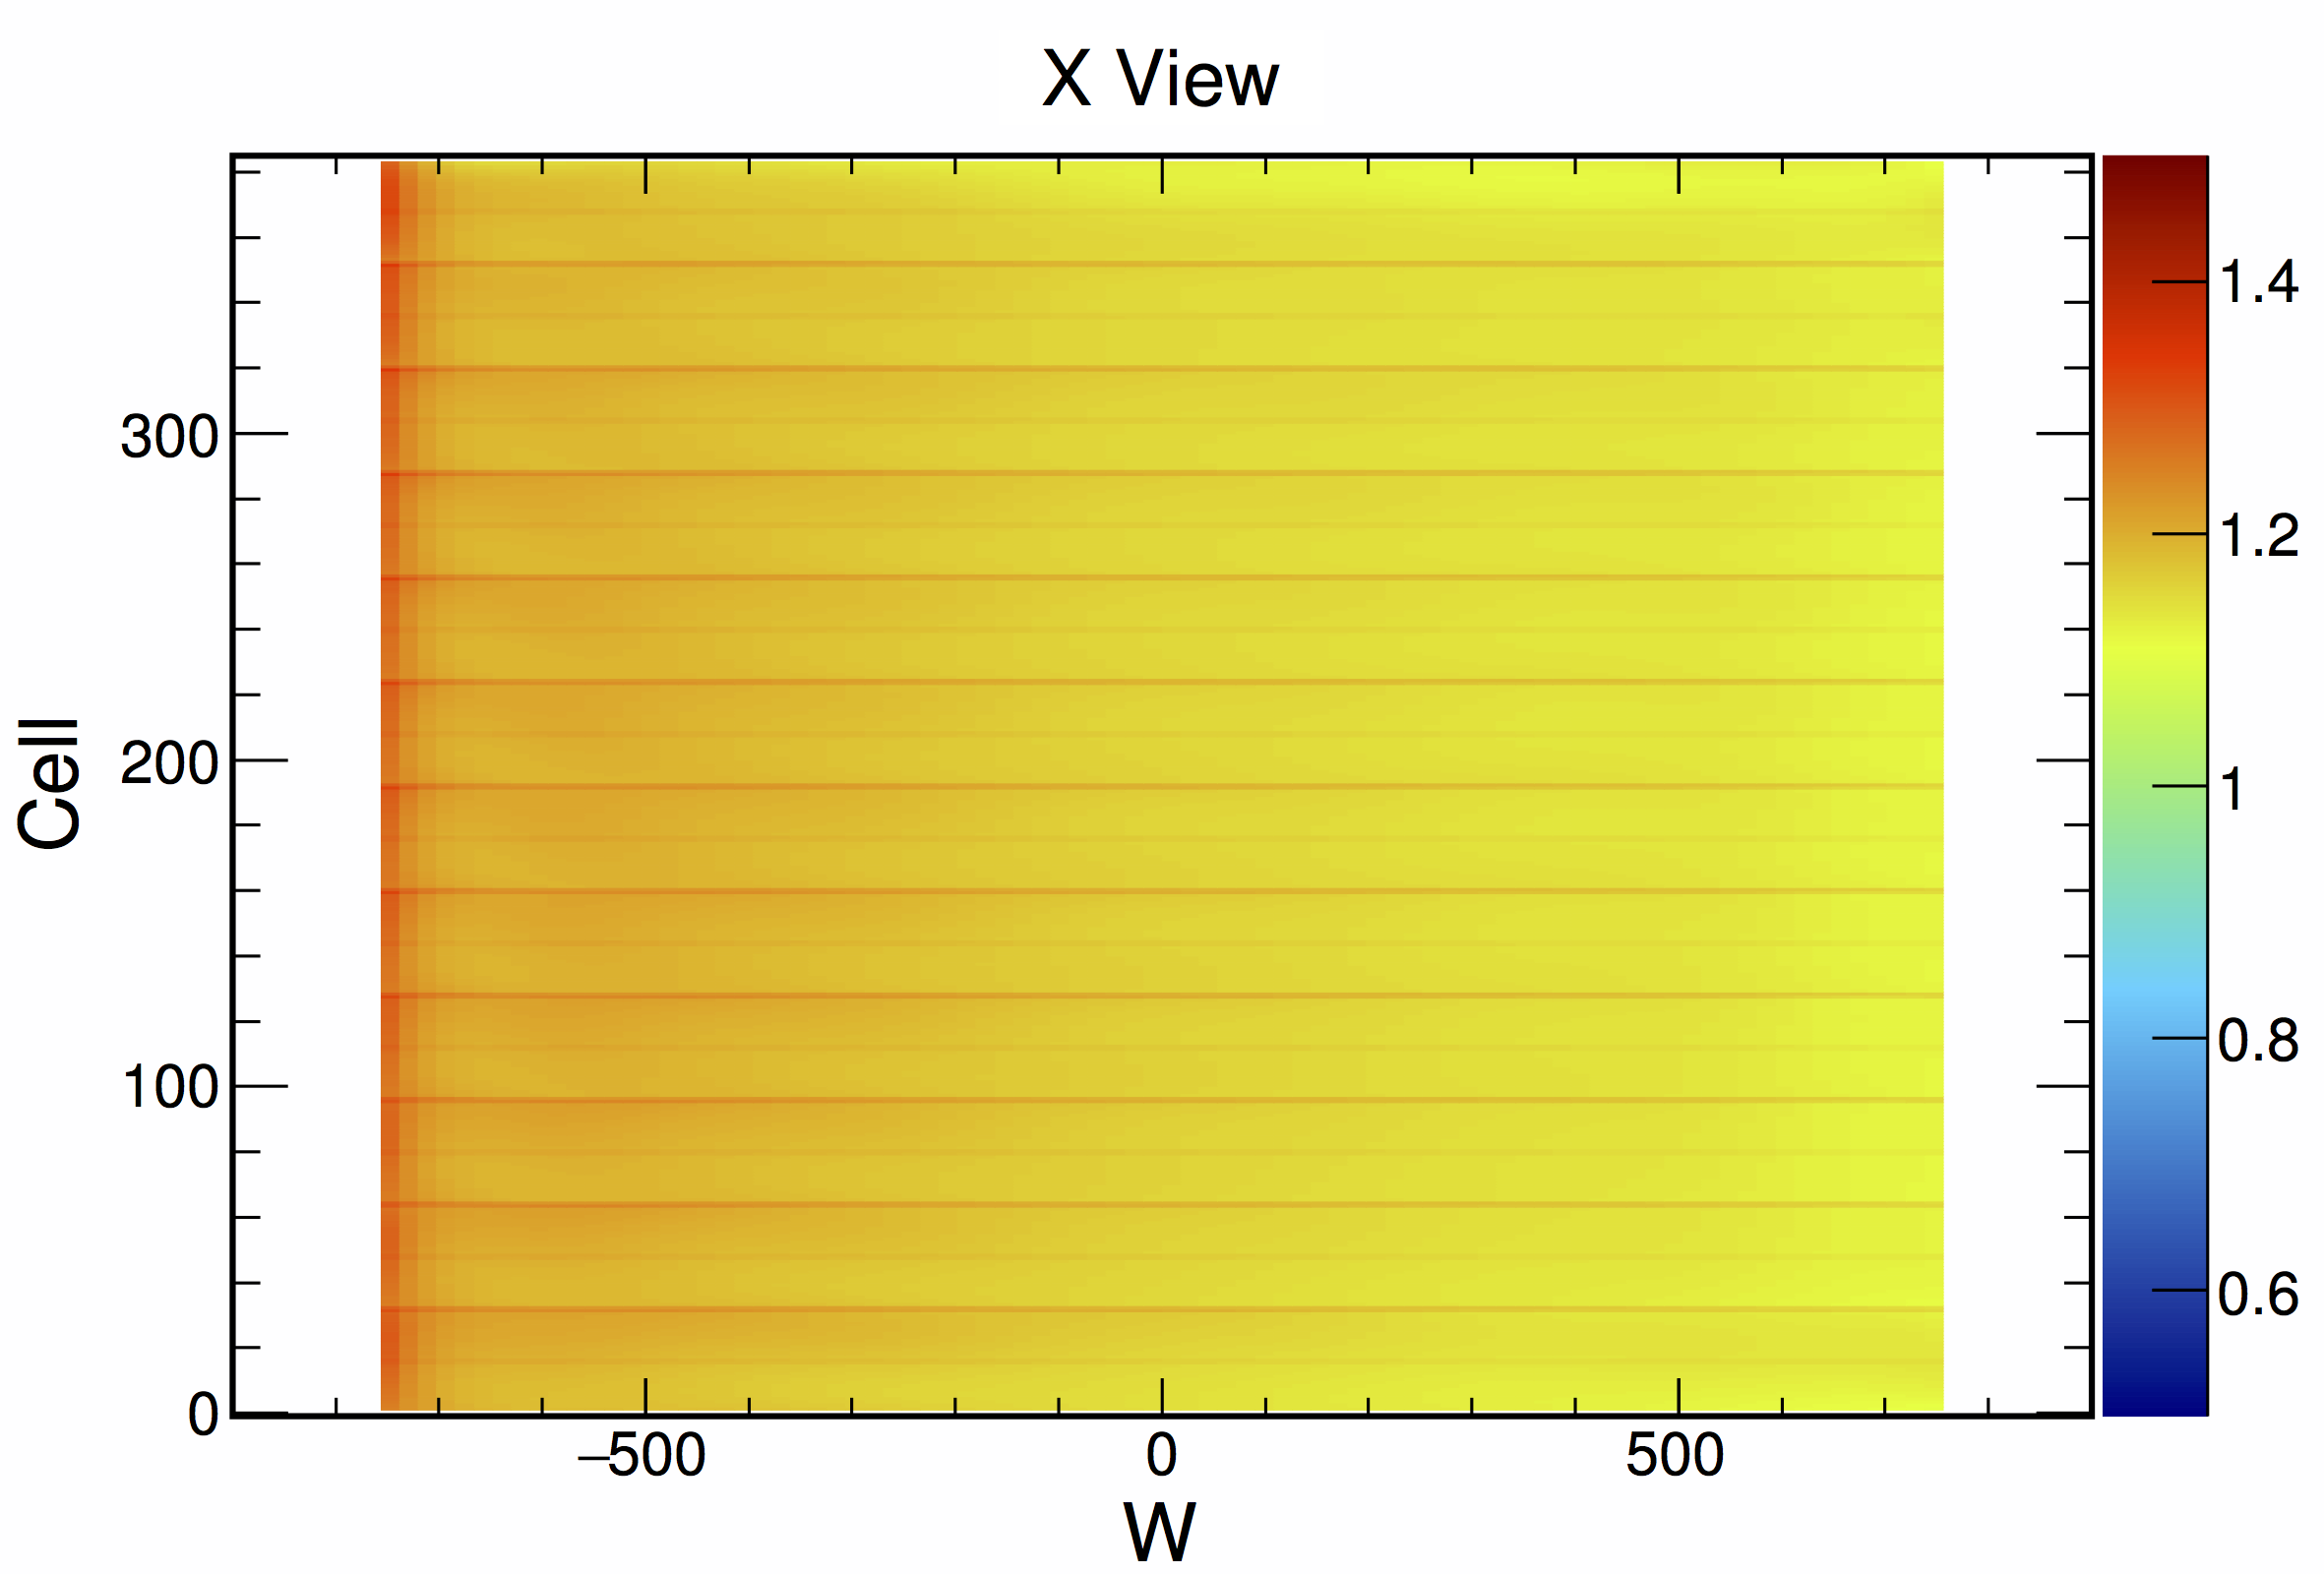
\includegraphics[width=.47\textwidth]{figures/Calib/ThresholdFDX.png} &
    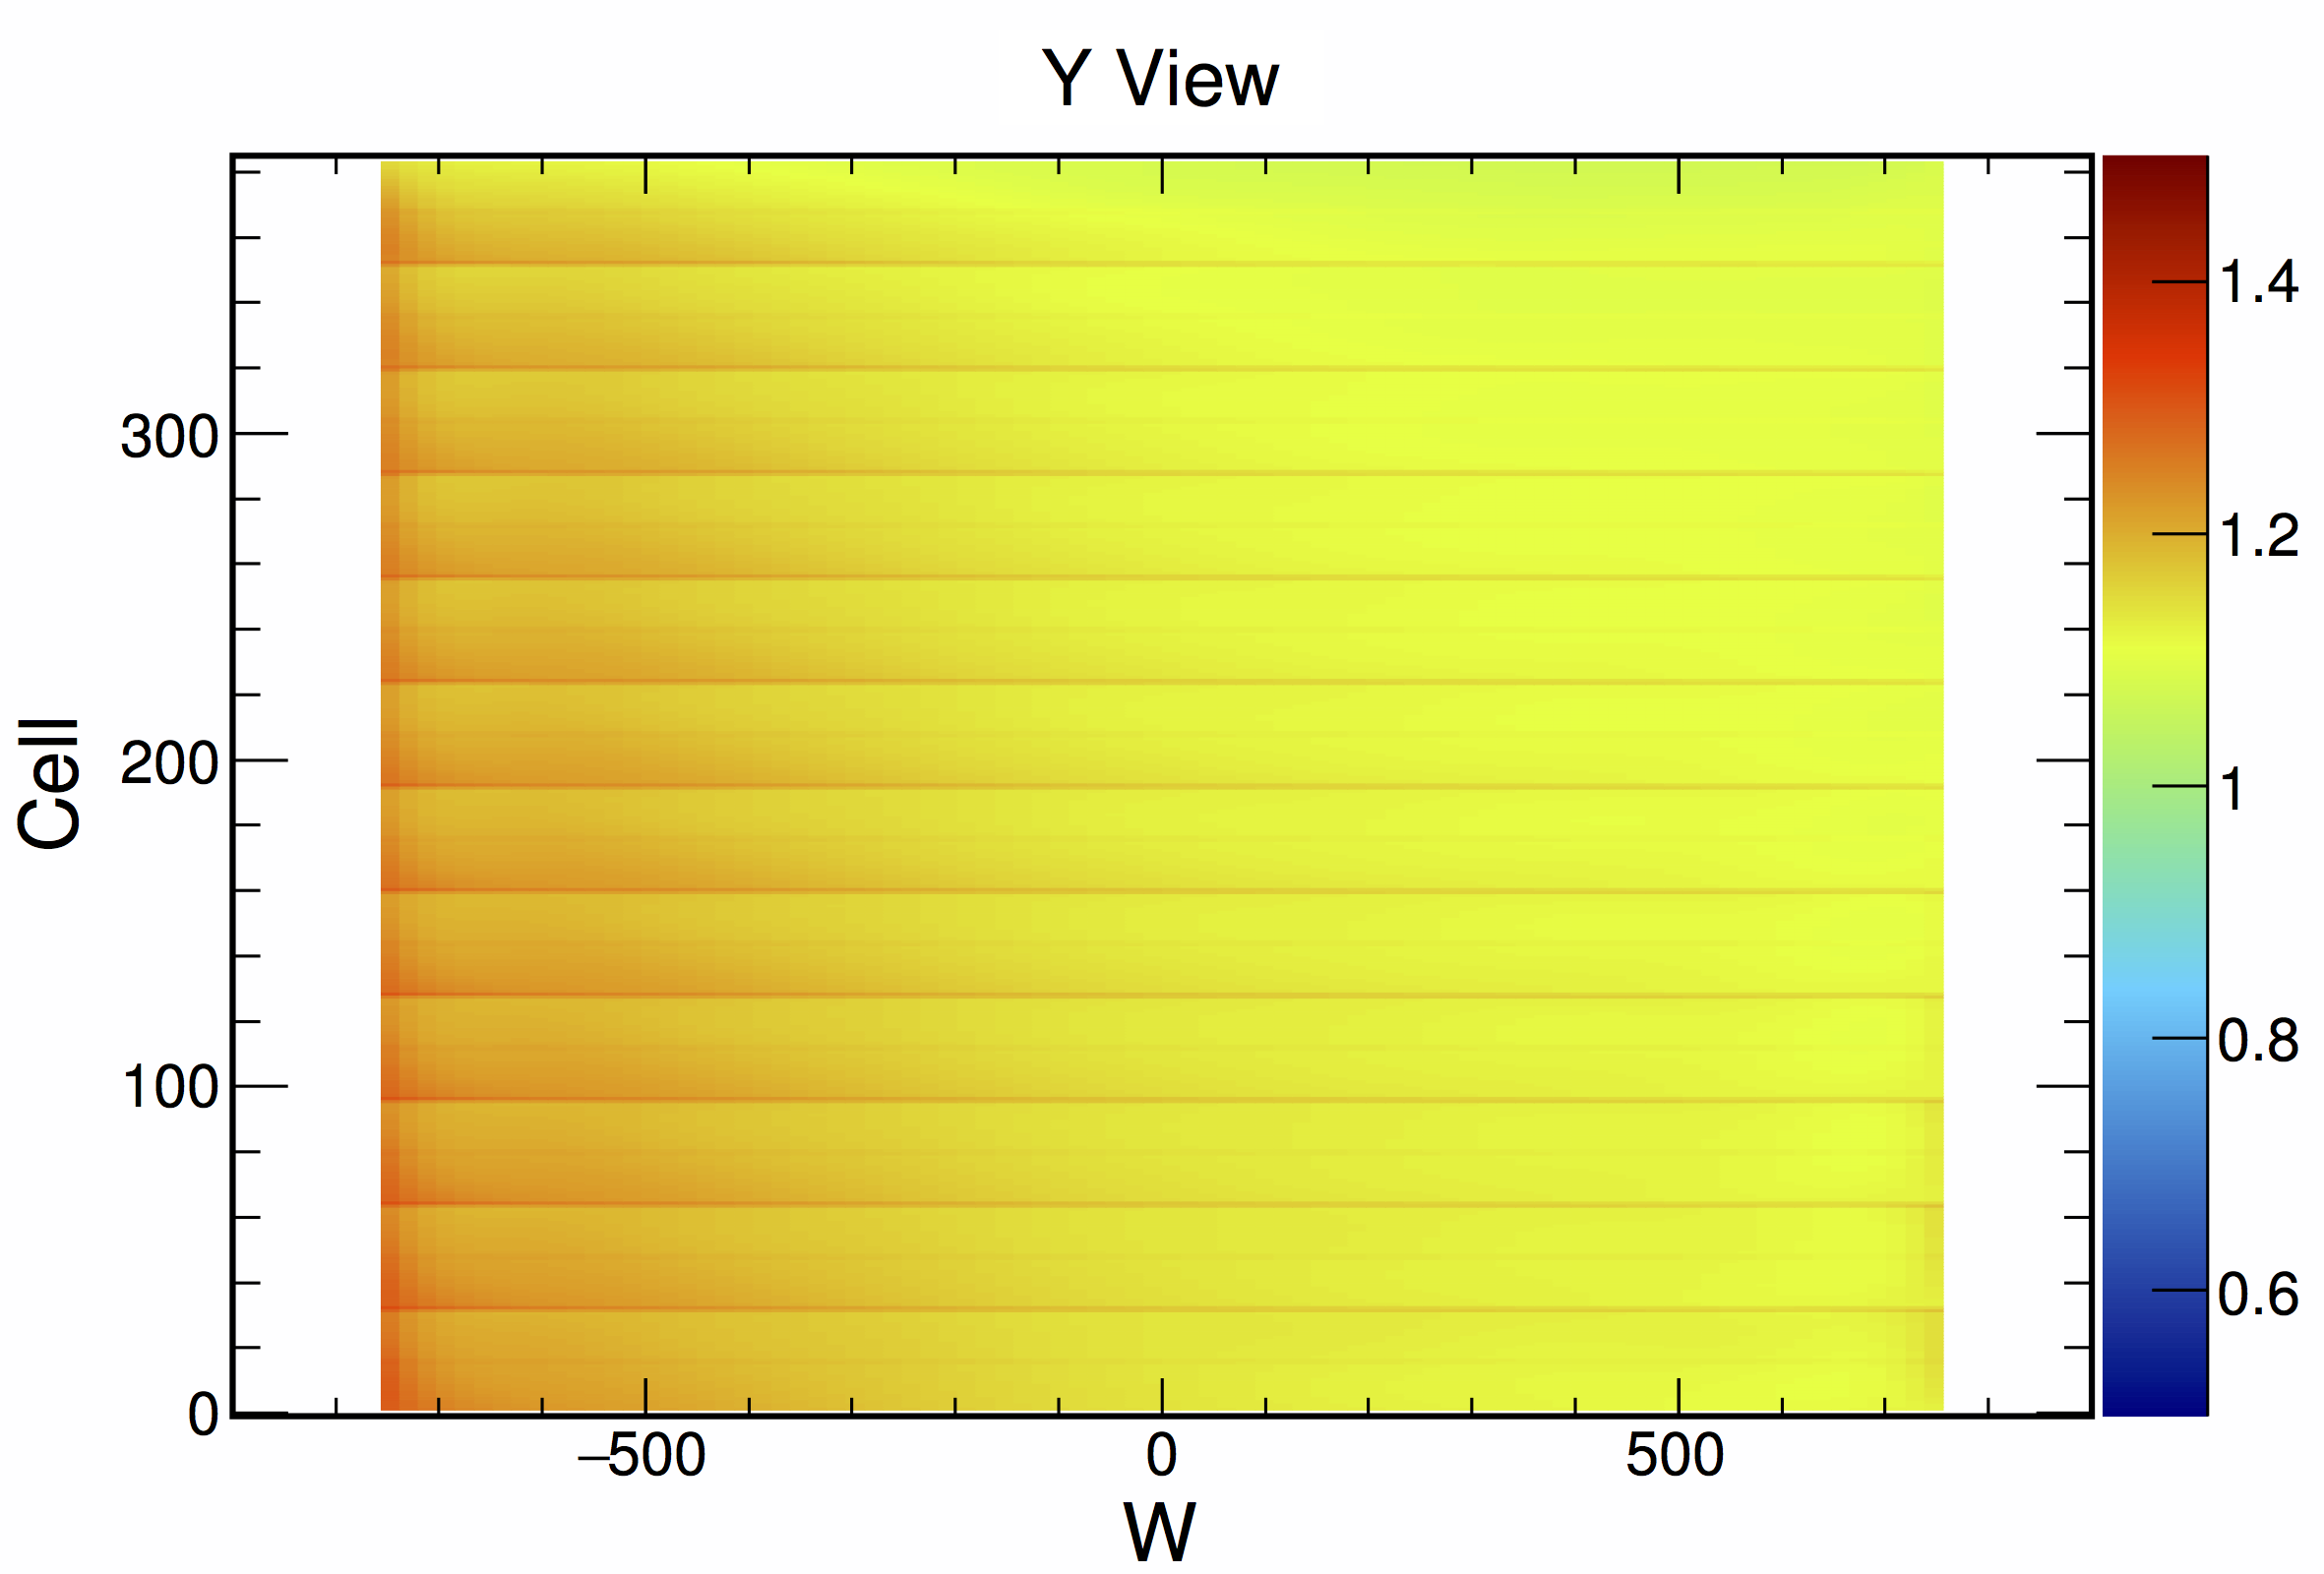
\includegraphics[width=.47\textwidth]{figures/Calib/ThresholdFDY.png} \\
  \end{tabular}
  \caption[Threshold and Shielding Correction Factors]{Correction factor for threshold and shielding effects at the FD as a function of cell number and distance from electronic readout. Cells in the X view are shown on the left, Y view on the right.}
  \label{fig:CalibThreshold}
\end{figure}

The next part of the relative calibration is the general form of the attenuation correction. Tricell hits are grouped by cell and fit to a double exponential to consider both short and long path light. For data, individual fits are performed for every single cell. In MC, a fit is performed on the group of all cells in a particular view and at the same location in a plane due to much lower simulated cosmic event statistics. The double exponential has the form
\beq
y = C + A\left(\exp\left(\frac{W}{X}\right) + \exp\left(-\frac{L+W}{X}\right)\right)
\label{eq:CalibAttenuation}
\eeq

\n where $C$, $A$, and $X$ are the free parameters, and $L$ is the full length of the cell. $X$ is the cell attenuation length. The fit excludes hits in the regions closest and furthest to the readout. It includes the range $[-750, 750]$ at the FD, $[-150, 150]$ for the fully active region of the ND and for Y view muon catcher cells, and $[-150, 50]$ for X view muon catcher cells, with all numbers in cm. These central regions are chosen to exclude the significant rolloff regions at the end of the cells, which are handled differently.

The final step in the relative calibration handles the attenuation correction at the ends of the cells and the residuals from the fit above in the central part of the cells. Both of these regions are fit with a single LOWESS curve using a tricube weight,
\beq
w_i = \begin{cases}
\left(1 - \left| \frac{W - W_i}{\sigma} \right|^3 \right)^3 & \mbox{for } \vert W - W_i \vert < \sigma \\
0 & \mbox{for } \vert W - W_i \vert \geq \sigma \end{cases}
\label{eq:CalibRolloff}
\eeq

\n where $W$ is a local point on the curve, $W_i$ is the $i$th neighbor of the local point, $w_i$ is the weight on $W_i$, and $\sigma = 30\unit{cm}$ is the range of neighbors that affect the value of $W$.

\section{Reconstruction Chain}
